% Created 2023-09-01 Fri 14:59
% Intended LaTeX compiler: pdflatex
\documentclass[11pt]{article}
\usepackage[utf8]{inputenc}
\usepackage[T1]{fontenc}
\usepackage{graphicx}
\usepackage{longtable}
\usepackage{wrapfig}
\usepackage{rotating}
\usepackage[normalem]{ulem}
\usepackage{amsmath}
\usepackage{amssymb}
\usepackage{capt-of}
\usepackage{hyperref}
\usepackage{tikz, siunitx}
\usetikzlibrary{patterns, shapes.geometric, calc}
\author{Hankertrix}
\date{\today}
\title{Newton's Laws of Motion Tutorial}
\hypersetup{
 pdfauthor={Hankertrix},
 pdftitle={Newton's Laws of Motion Tutorial},
 pdfkeywords={},
 pdfsubject={},
 pdfcreator={Emacs 29.1 (Org mode 9.6.6)}, 
 pdflang={English}}
\begin{document}

\maketitle
\setcounter{tocdepth}{2}
\tableofcontents

\newpage

\section{Question 1}
\label{sec:org606c7bf}
The net force that the length of the chain x experiences is:
\[F_{net} = (l-x)w - xw\]
\[F_{net} = w(l-2x)\]

Since the \(F_{net} = ma\):
\[ma = w(l-2x)\]
\[a = \frac{w(l-2x)}{\frac{lw}{g}}\]
\[a = \frac{g(l-2x)}{l}\]

\section{Question 2}
\label{sec:orgafb6b97}

\subsection{(a)}
\label{sec:orgbfab878}
The weight of the block is vertically downwards, which means it cannot provide for the horizontal acceleration of the block. This means that the normal contact force of the slope on the block must be providing for the horizontal acceleration of the block.
\\[0pt]

The vertical component of the normal contact force of the slope on the block is \(mg\). Hence, the normal contact force of the slope on the block is \(\frac{mg}{\cos \theta}\).
\\[0pt]

The horizontal component of the normal contact force of the slope on the block provides for the acceleration of the block, so the horizontal acceleration of the block would be:
\[a = \frac{F_{net}}{m}\]
\[a = \frac{\left(\frac{mg}{\cos \theta} \right) \sin \theta}{m}\]
\[a = \frac{\frac{mg \sin \theta}{\cos \theta}}{m}\]
\[a = \frac{mg \tan \theta}{m}\]
\[a = g \tan \theta\]

For the block to stay still relative to the wedge, the wedge will have to counteract this acceleration, so the wedge will have to accelerate at \(g \tan \theta\).

\subsection{(b)}
\label{sec:org75fd73c}

The horizontal force required would be the total mass of the wedge and the block multiplied by the acceleration needed, which is \((M + m)g \tan \theta\).

\subsection{(c)}
\label{sec:orge504ae2}

The block will move down the slope as usual. Using Newton's third law, when the wedge exerts a force on the block (the normal contact force), the block will exert an equal and opposite force on the wedge. Since there is no friction to keep the wedge in place, the wedge will move horizontally leftwards while the block moves down the slope.

\section{Question 3}
\label{sec:org898bb50}

\subsection{(a)}
\label{sec:org5a21cd5}
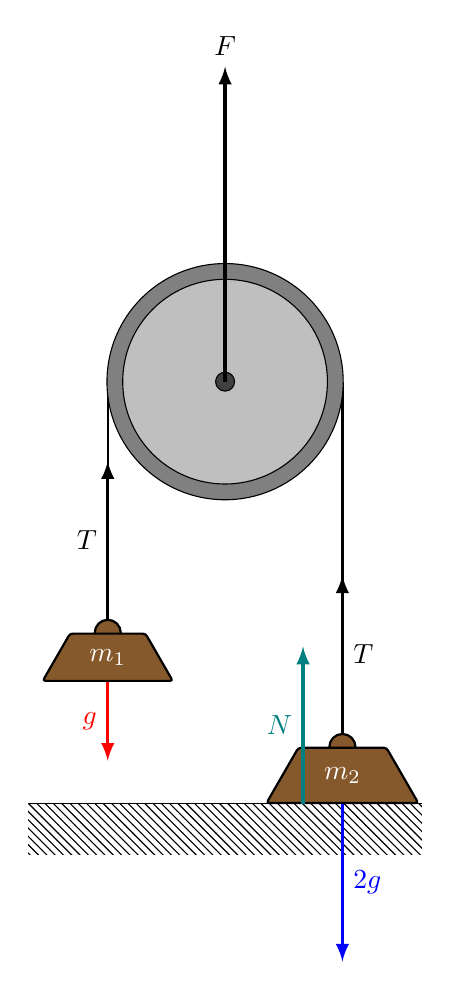
\begin{tikzpicture}

% Mass 1
\draw[thick] (-1.49cm,0) -- ++(0,-3.5cm) node[draw=black,above=0.13cm,circle,fill=brown!70!black](cm){} node[draw=black,trapezium,rounded corners=1pt,fill=brown!70!black,text=white, minimum height=0.6cm](m){$m_1$};

% Mass 2
\draw[thick] (1.49cm,0) -- ++(0,-5cm) node[draw=black,above=0.18cm,circle,fill=brown!70!black](cM){}
node[draw=black,trapezium,rounded corners=1pt,fill=brown!70!black,text=white, minimum height=0.7cm](M){$m_2$};

% Supporting structure
\fill[pattern= north west lines,] (-2.5,-5.36) rectangle (2.5,-6);
\draw(-2.5,-5.36) -- (2.5,-5.36);

% Pulley
\draw[fill = gray] (0,0) circle (1.5cm); % Big circle
\draw[fill=lightgray] (0,0) circle (1.3cm); % Medium circle
\draw[fill=darkgray] (0,0) circle (0.12cm); % Axle circle

% Forces on the pulley
\draw[-latex, very thick, black] (0,0) -- ++(0,4) node[above]{$F$};

% Forces on mass 1
\draw [-latex,very thick,red] (m.bottom side) -- ++(0,-1) node[midway,left]{$g$};
\draw [-latex,very thick,black] (cm.north) -- ++(0,2) node[midway,left]{$T$};

% Forces on mass 2
\draw [-latex,very thick,blue] (M.bottom side) -- ++(0,-2) node[midway,right]{$2g$};
\draw [-latex,very thick,black] (cM.north) -- ++(0,2) node[midway,right]{$T$};
\draw[-latex,very thick,teal] ($ (M.bottom side) + (-0.5,0) $) -- ++(0,2) node[midway, left]{$N$};

\end{tikzpicture}

\newpage

\subsection{(b)}
\label{sec:orge9dc0d8}

The tension in the string will need to counteract the weight of the mass \(m_2\) since the normal contact force is zero when mass \(m_2\) doesn't leave the ground. Hence:
\[T = 2g\]
\\[0pt]

Since \(F = 2T\):
\[F = 2T\]
\[F = 2 \times 2g\]
\[F = 4g\]
\[F = 39.24\]
\[F = 39.3 \si{N} \text{ (3 s.f)}\]

\subsection{(c)}
\label{sec:orgb193e45}

Since \(F = 2T\), the tension in the string would be:
\[2T = F\]
\[T = \frac{F}{2}\]
\[T = \frac{100}{2}\]
\[T = 50 \si{N}\]

\subsection{(d)}
\label{sec:org634addd}
The net force on mass \(m_1\) would be:
\begin{align*}
T - m_1g &= 50 - 1g \\
&= 50 - 9.81 \\
&= 40.19 \si{N}
\end{align*}

Hence, the acceleration of the mass \(m_1\) would be:
\[F = ma\]
\[40.19 = 1a\]
\[a = 40.19\]
\[a = 40.2 \si{ms^{-2}} \text{ (3 s.f)}\]


\section{Question 4}
\label{sec:org39a4893}

\subsection{(a)}
\label{sec:org343fe40}
When the elevator descents at constant speed, there's no acceleration due to the elevator as the net force on the block does not change and hence the block will accelerate down the slope at \(g \sin \theta\).

\subsection{(b)}
\label{sec:orge84b257}
When the elevator ascends at constant speed, there's again no acceleration due to the elevator as the net force on the block does not change and hence the block will accelerate down the slope at \(g \sin \theta\) as well.

\subsection{(c)}
\label{sec:orgbcab712}
When the elevator descends with acceleration, the vertical component of the normal contact force of the incline on the block decreases by \(ma\), which means the net force on the block will be \((mg - ma)\). Since \(F = ma\), the acceleration of the block down the incline will be:
\begin{align*}
a &= \frac{F_{net}}{m} \sin \theta \\
&= \frac{mg - ma}{m} \sin \theta \\
&= (g - a) \sin \theta \\
\end{align*}

\subsection{(d)}
\label{sec:orgd65eda7}
When the elevator ascends with acceleration, the vertical component of the normal contact force of the incline on the block increases by \(ma\), which means the net force on the block will be \((mg + ma)\). Since \(F = ma\), the acceleration of the block down the incline will be:
\begin{align*}
a &= \frac{F_{net}}{m} \sin \theta \\
&= \frac{mg + ma}{m} \sin \theta \\
&= (g + a) \sin \theta \\
\end{align*}

\subsection{(f)}
\label{sec:org1beb01d}
Since we have already found the vertical component of the normal contact force of the incline on the block to be \(mg - ma\), the normal contact force of the incline on the block will be:
\begin{align*}
N &= (mg - ma) \cos \theta \\
&= m(g - a) \cos \theta
\end{align*}

\section{Question 5}
\label{sec:orgc07145e}

\subsection{(a)}
\label{sec:orge8c52b2}
The weight of the box will be \(mg\) which is:
\begin{align*}
mg &= 20 \times 9.81 \\
&= 196.2 \\
&= 196 \si{N} \text{ (3 s.f)}
\end{align*}

By Newton's Third Law, the normal contact force of the table on the box will be equal and opposite to the weight of the box on the table, hence the normal contact force acting on the box will be equal in magnitude to the weight, which is \(196 \si{N} \text{ (3 s.f)}\).

\subsection{(b)}
\label{sec:org1947721}
By Newton's Third Law, the normal contact force of the table will be equal and opposite to the total weight of the boxes on the table. Hence, the normal contact force of the table on the \(20.0 \si{kg}\) box will be:
\begin{align*}
N &= (10 + 20)(9.81) \\
&= 30 \times 9.81 \\
&= 294.3 \si{N} \\
&= 294 \si{N} \text{ (3 s.f)}
\end{align*}

\newpage

\subsection{(c)}
\label{sec:org40ce0ee}
By Newton's Third Law, the normal contact force of the \(20.0 \si{kg}\) box on the \(10.0 \si{kg}\) box will be equal and opposite to the weight of the \(10.0 \si{kg}\) box placed on top of it. Hence, the normal contact force of the \(20.0 \si{kg}\) box will be:
\begin{align*}
N &= 10 \times 9.81 \\
&= 98.1 \si{N}
\end{align*}
\end{document}